\chapter{Analysis of musical concepts learned by the model}
% **************************** Define Graphics Path **************************
\ifpdf
    \graphicspath{{Chapter5/Figs/Raster/}{Chapter5/Figs/PDF/}{Chapter5/Figs/}}
\else
    \graphicspath{{Chapter5/Figs/Vector/}{Chapter5/Figs/}}
\fi

\section{Investigation of neuron activation responses to applied stimulus}

One method for gaining insight into what a connectionist model has learned is
to apply some stimulus and measure neuron activations at different layers.

We use as stimulus the music score shown in
\cref{fig:model-analysis-stimulus}, which has been preprocessed according to
\mynote{cite preprocessing}. To aid in relating neuron activities back to music
theory, chords are annotated with Roman numerals obtained using {\tt music21}'s
automated analysis.

\begin{figure}[tb]
    \centering
    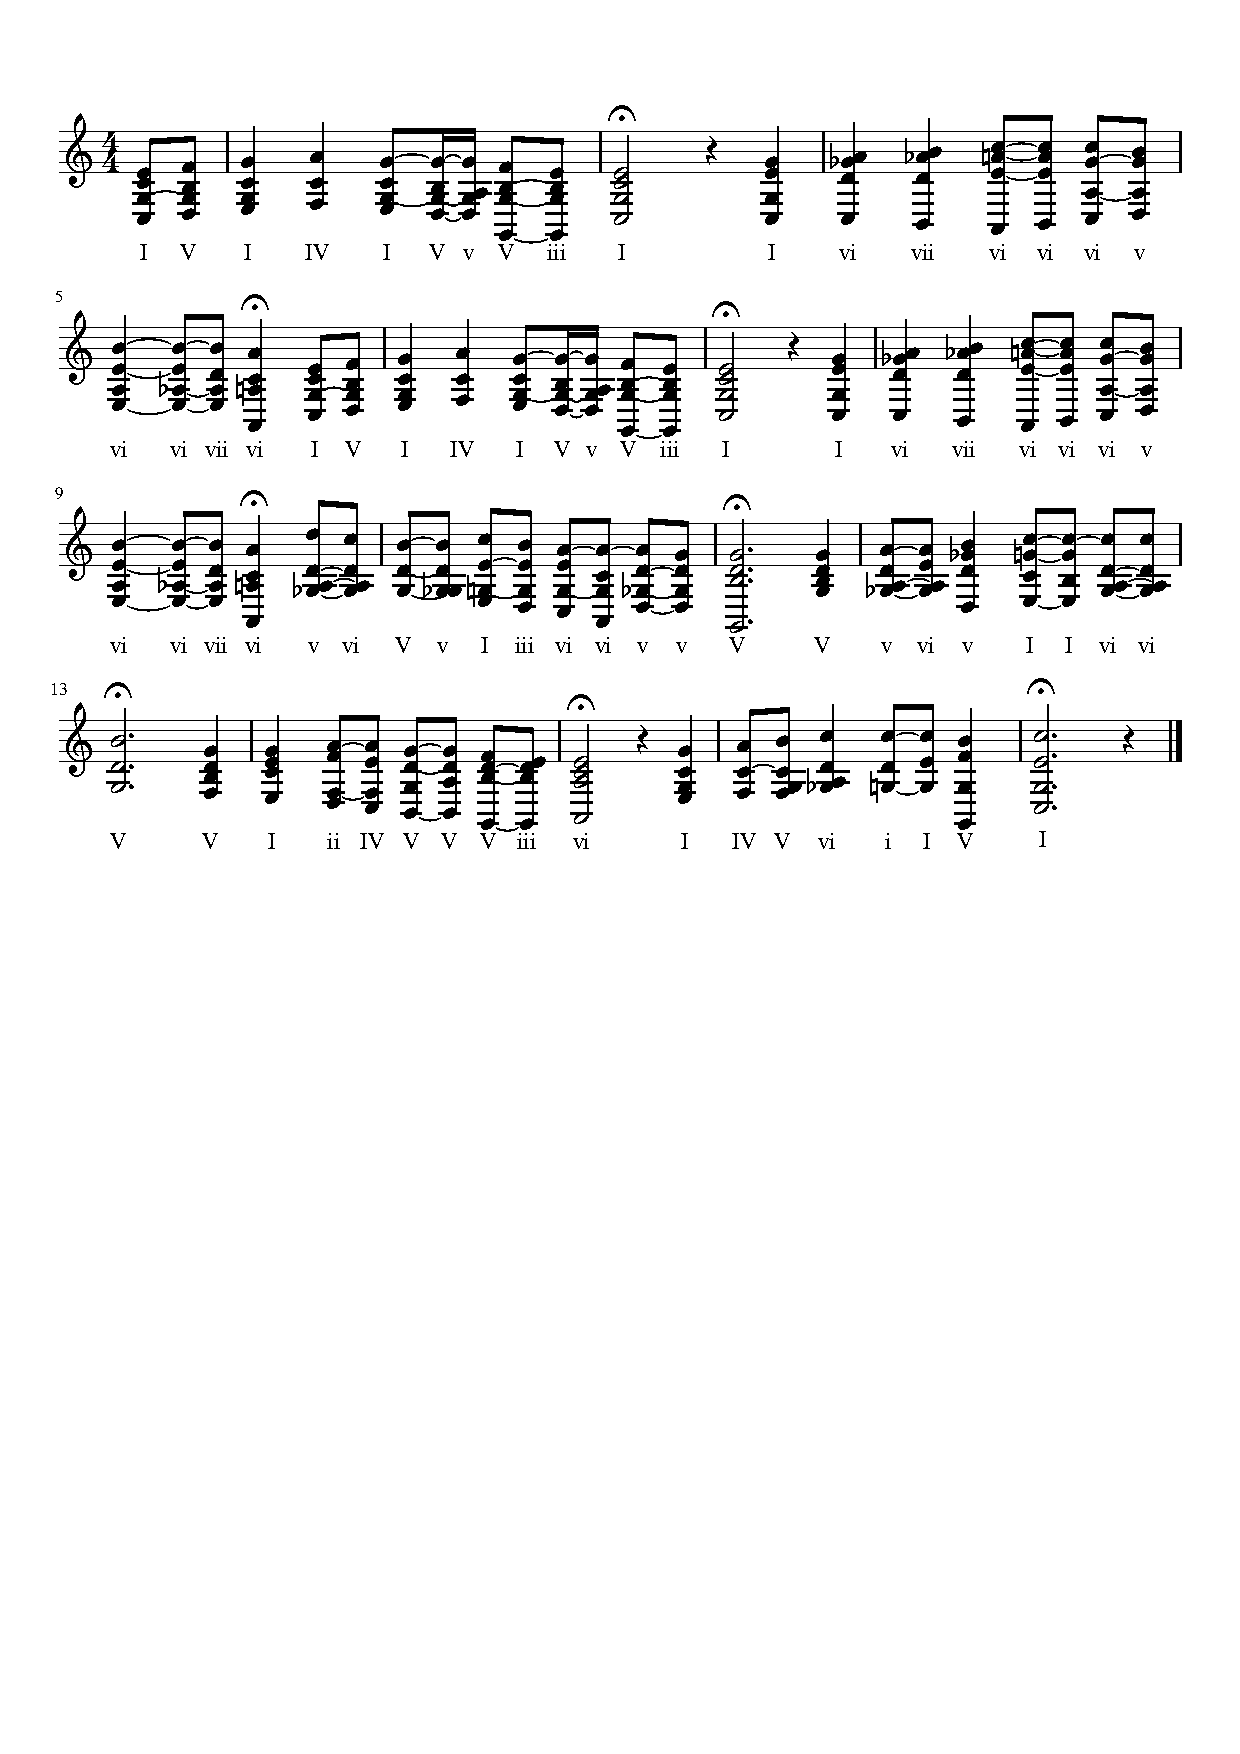
\includegraphics[trim={0 15cm 0 0},clip,width=0.9\linewidth]{model-analysis-input-score.pdf}
    %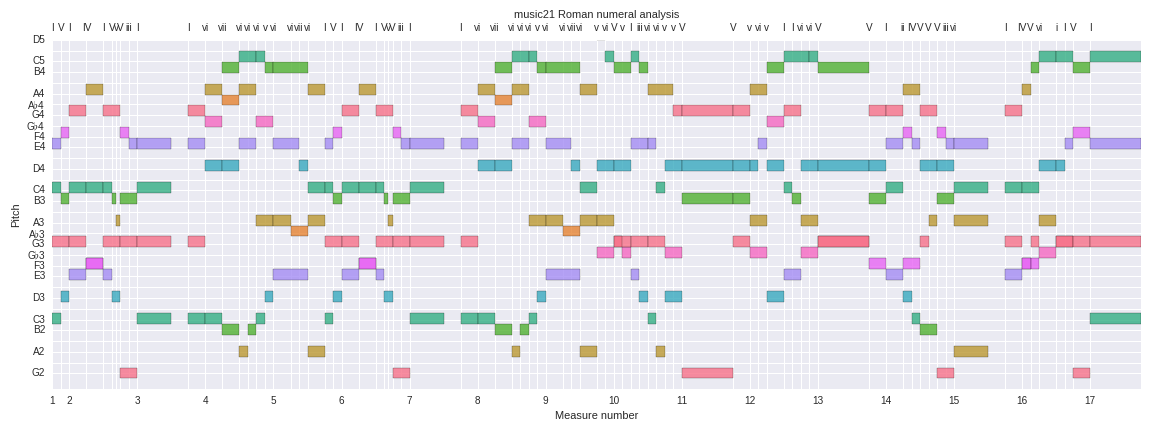
\includegraphics[width=1.00\linewidth]{model-analysis-input-piano-roll.png}
    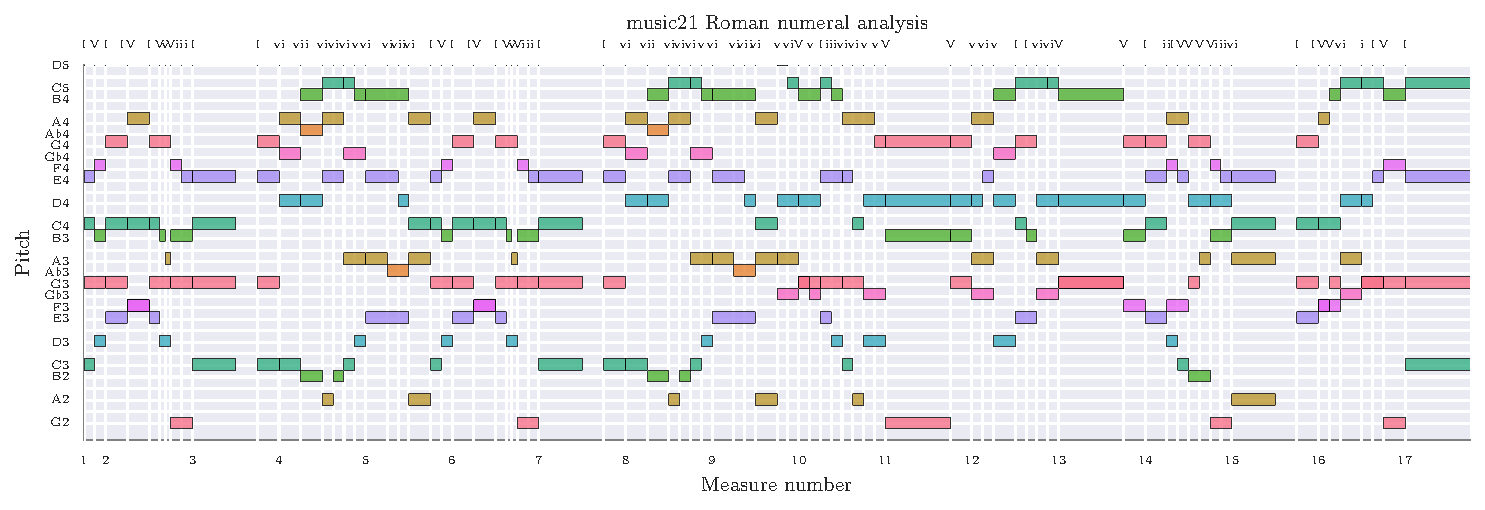
\includegraphics[width=1.00\linewidth]{model-analysis-input-piano-roll.pdf}
    %\input{Chapter5/Figs/model-analysis-input-piano-roll.pgf}
    \caption{{\it Top}: The preprocessed score (BWV 133.6) used as input stimulus with Roman numeral analysis annotations obtained
        from {\tt music21}; {\it Bottom}: The same stimulus represented on a piano roll}
    \label{fig:model-analysis-stimulus}
\end{figure}

In \cref{fig:model-analysis-tokens} we visualize the network activations as
the stimulus is sequentially applied. Note that as a consequence of the
variable-length encoding format described in \mynote{ref}, the horizontal axis
(number of tokens processed) does correspond directly to time. Rather, time
is advanced one frame every time a chord boundary delimiter symbol is output.

\begin{figure}[tb]
    \centering
    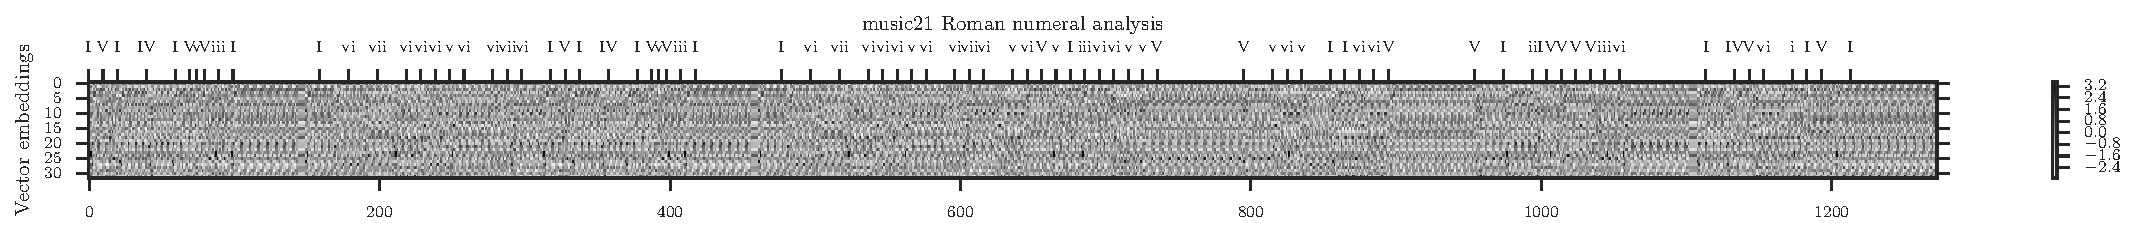
\includegraphics[width=1.0\linewidth]{model-analysis-tokens-0.pdf}
    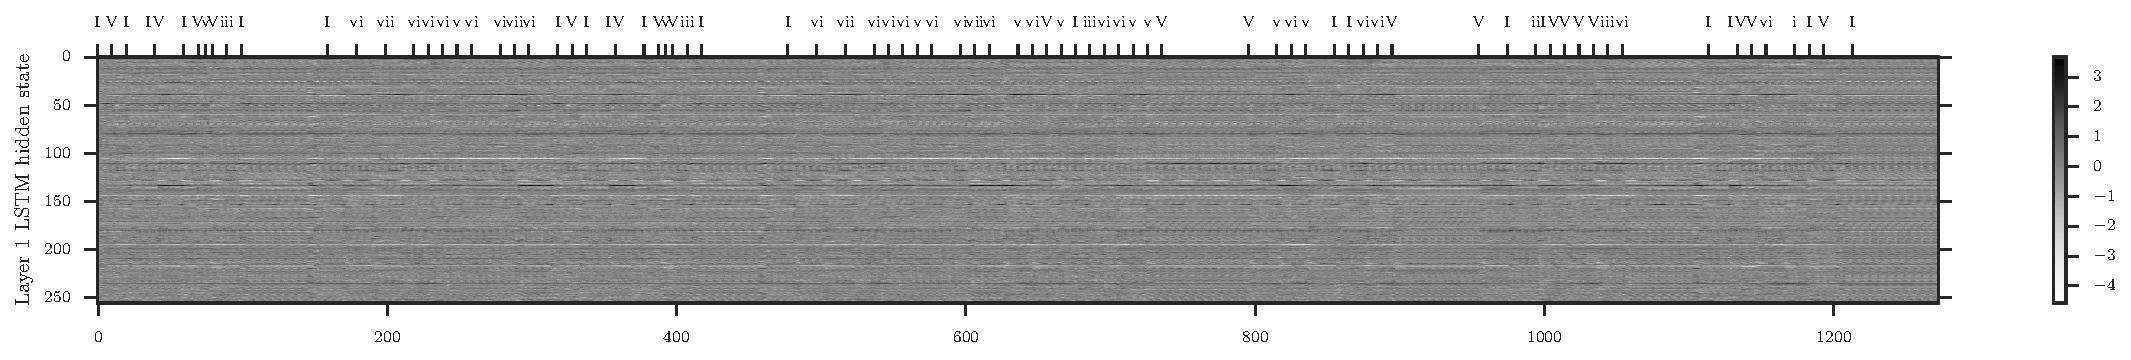
\includegraphics[width=1.0\linewidth]{model-analysis-tokens-1.pdf}
    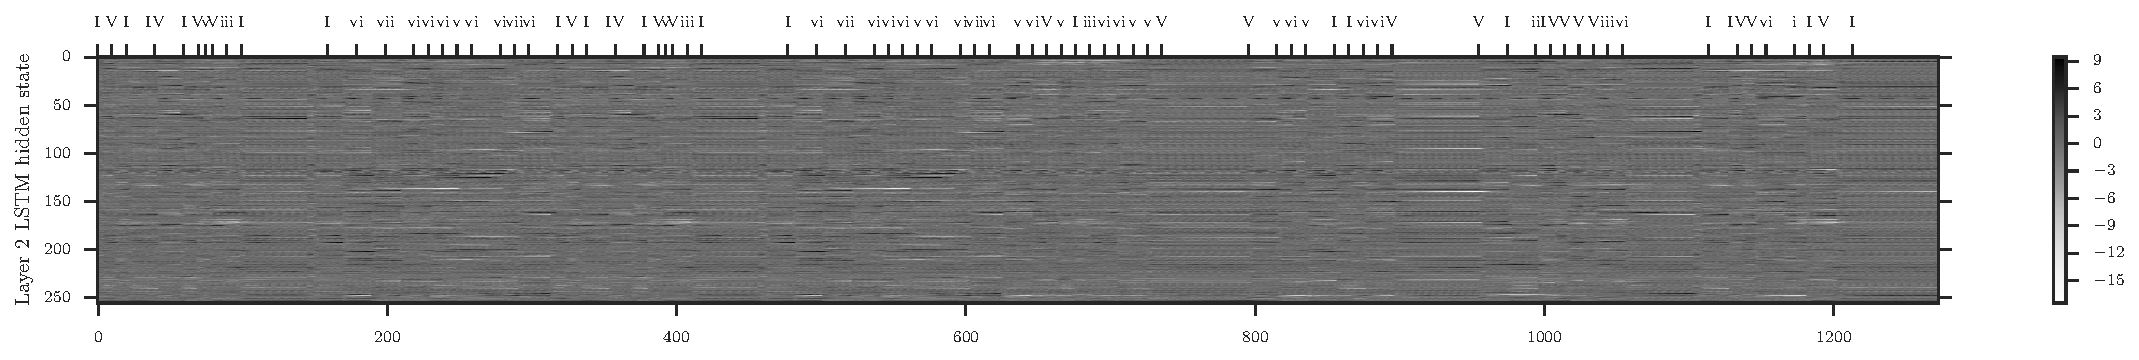
\includegraphics[width=1.0\linewidth]{model-analysis-tokens-2.pdf}
    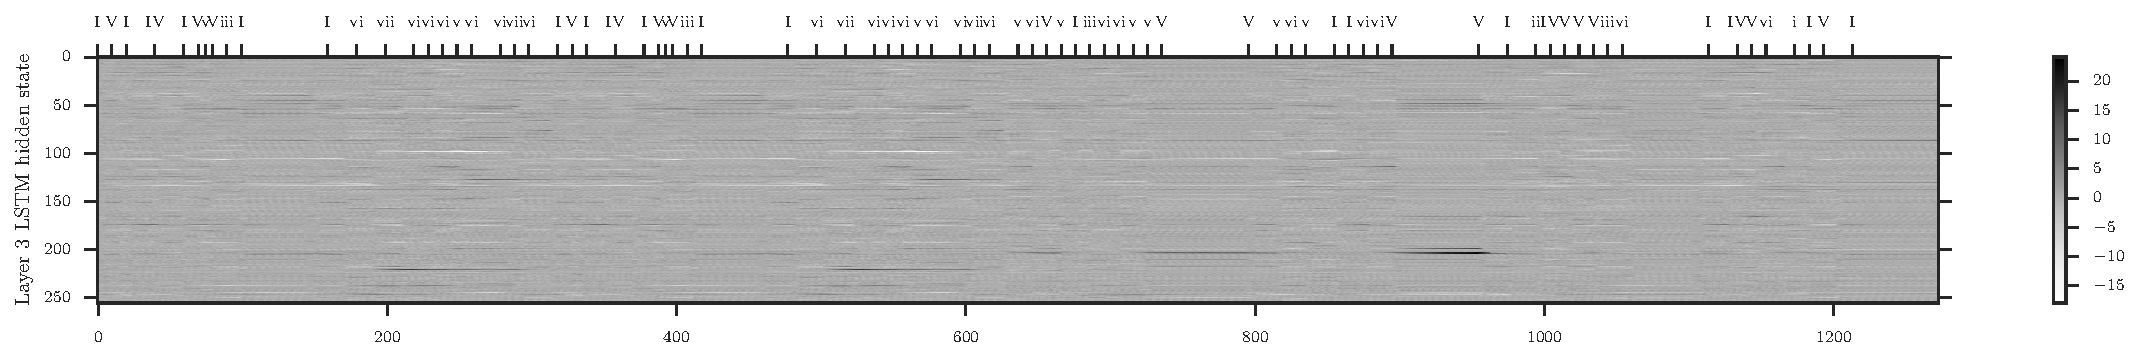
\includegraphics[width=1.0\linewidth]{model-analysis-tokens-3.pdf}
    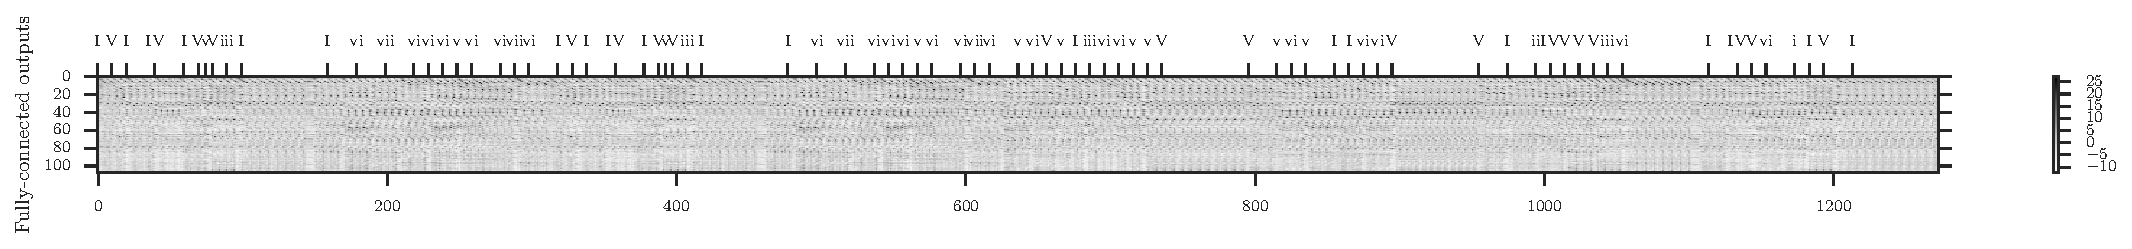
\includegraphics[width=1.0\linewidth]{model-analysis-tokens-4.pdf}
    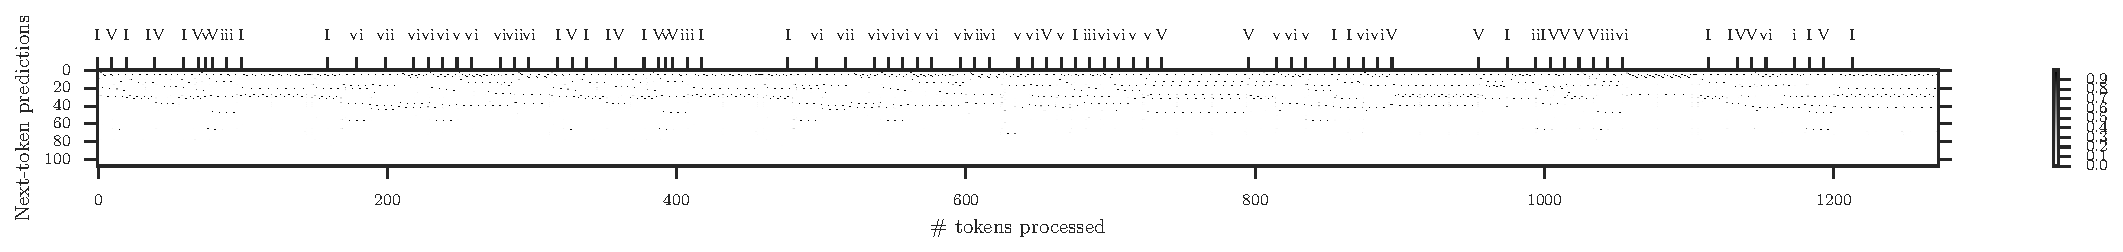
\includegraphics[width=1.0\linewidth]{model-analysis-tokens-5.pdf}
    \caption{Neuron activations over time as the encoded stimulus is processed token-by-token}
    \label{fig:model-analysis-tokens}
\end{figure}

\subsection{Pooling over frames}

In order to align and compare the activation profiles with the original score,
all the activations occuring in between two chord boundary delimiters must be
combined. This aggregation of neuron activations from higher resolution (\ie
note-by-note) to lower resolution (\ie frame-by-frame) is reminiscent of
pooling operations in convolutional neural networks\mynote{cite}. Motivated by
this observation, we introduce the method for pooling an arbitrary number of
token-level activations into a single frame-level activation.

Let $\z^{(l)}_{{t_m}:{t_n}}$ denote the activations of layer $l$ from the $t_m$th input token $\x_{t_m}$
to the $t_n$th input token $\x_{t_n}$. Suppose that $\x_{t_m}$ and $\x_{t_n}$ are respectively the
$m$th and $n$th chord boundary delimiters within the input sequence. Define the
\textbf{max-pooled frame-level activations} $\tilde{\z}^{(l)}_n$ to be the
element-wise maximum of $\z^{(l)}_{{t_m}:{t_n}}$, that is:
\begin{equation}
    \tilde{\z}^{(l)}_n \coloneqq \left[
        \max_{t_m < t < t_n} \z^{(l)}_{t,1},\quad
        \max_{t_m < t < t_n} \z^{(l)}_{t,2},\quad
        \cdots,\quad
        \max_{t_m < t < t_n} \z^{(l)}_{t,N^{(l)}}
    \right]^\tp
\end{equation}
where $\z^{(l)}_{t,i}$ is the activation of neuron $i$ in layer $l$ at time $t$
and $N^{(l)}$ is the number of neurons in layer $l$. Notice that the pooled
sequence $\tilde{\z}$ is now indexed by frames rather than by tokens and hence
corresponds to time-steps.

We choose to perform max pooling because it preserves the maximum activations
of each neuron over the frame. While pooling methods (\eg sum pooling, average
pooling) are possible, we did not find significant differences in the
visualizations produced.

The max-pooled frame-level activations are shown in
\cref{fig:model-analysis-frames}. As a result of pooling, the horizontal axis
can be aligned and compared against the stimulus
\cref{fig:model-analysis-stimulus}. Notice the appearance of vertical bands
corresponding to when a chord/rest is held for multiple frames. In particular,
the vector embedding corresponding to rests (\eg near frames $30$ and $90$ in
\cref{fig:model-analysis-frames} top) are sparse, showing up as white smears
not only in the embedding layer but on all LSTM memory cells.

\begin{figure}[tb]
    \centering
    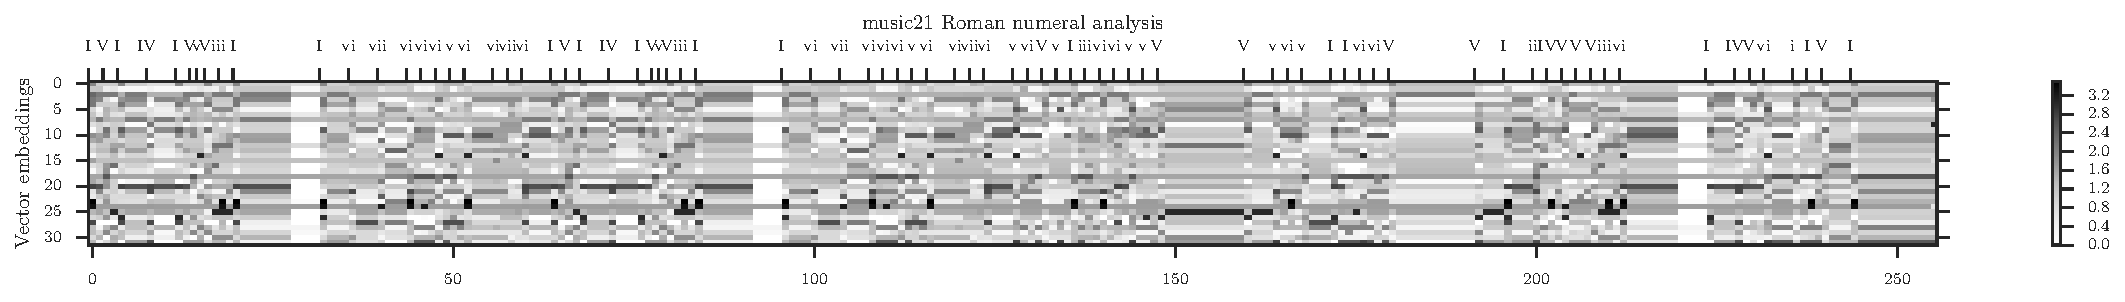
\includegraphics[width=1.0\linewidth]{model-analysis-chords-0.pdf}
    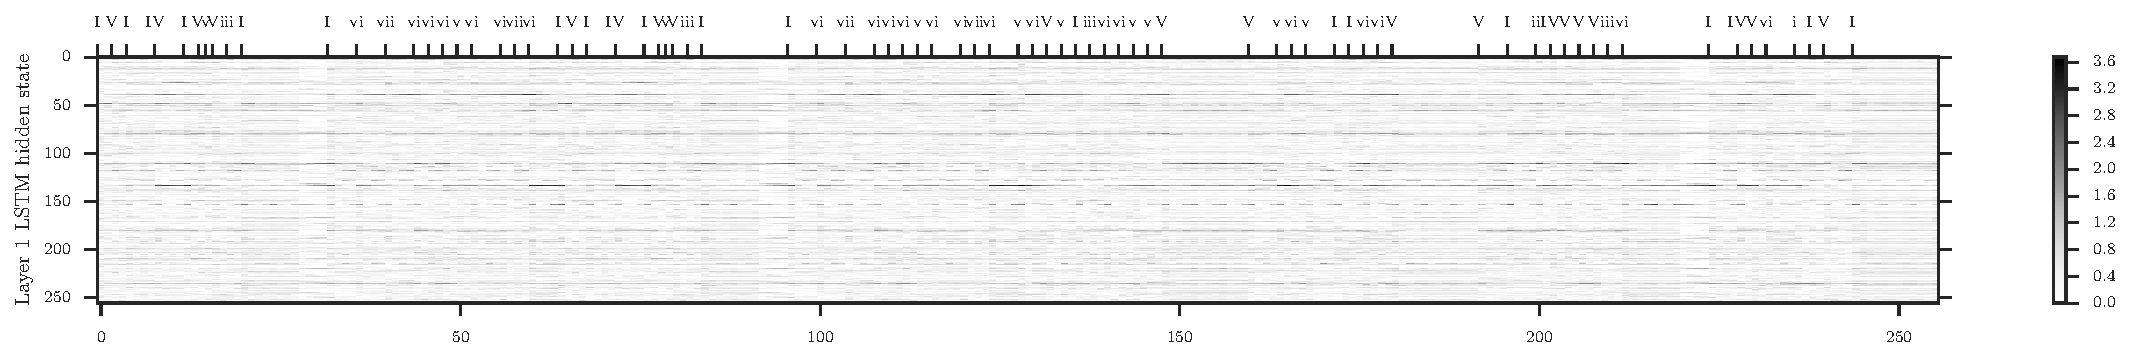
\includegraphics[width=1.0\linewidth]{model-analysis-chords-1.pdf}
    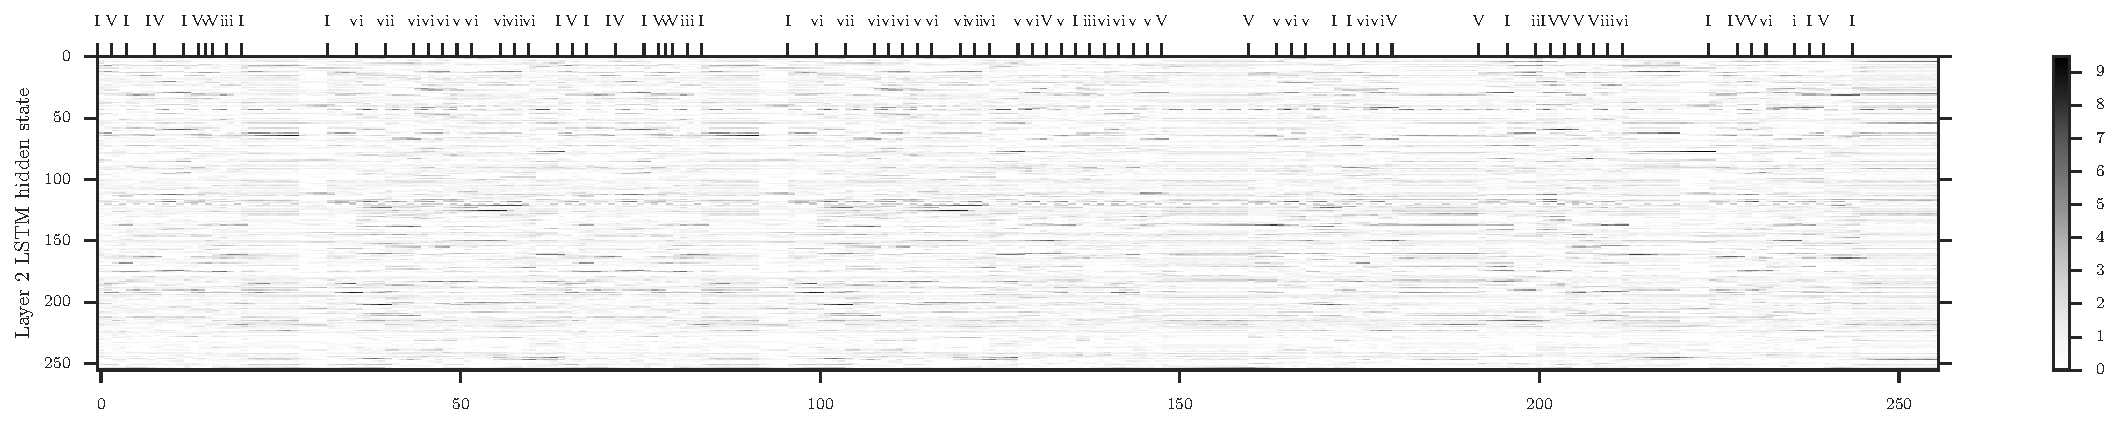
\includegraphics[width=1.0\linewidth]{model-analysis-chords-2.pdf}
    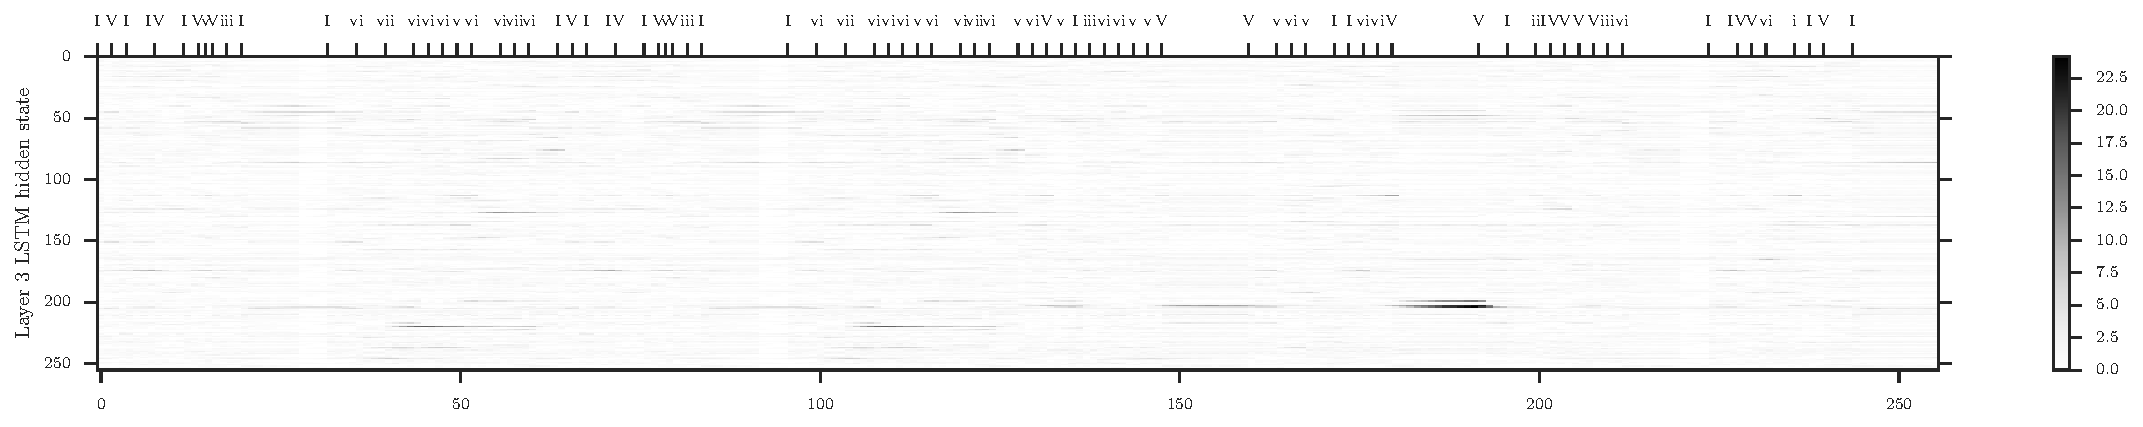
\includegraphics[width=1.0\linewidth]{model-analysis-chords-3.pdf}
    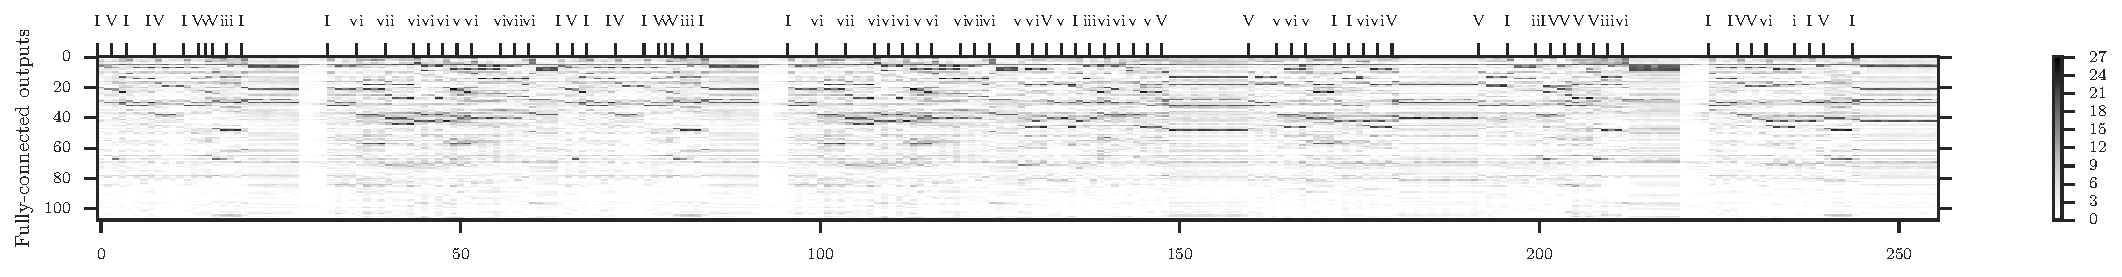
\includegraphics[width=1.0\linewidth]{model-analysis-chords-4.pdf}
    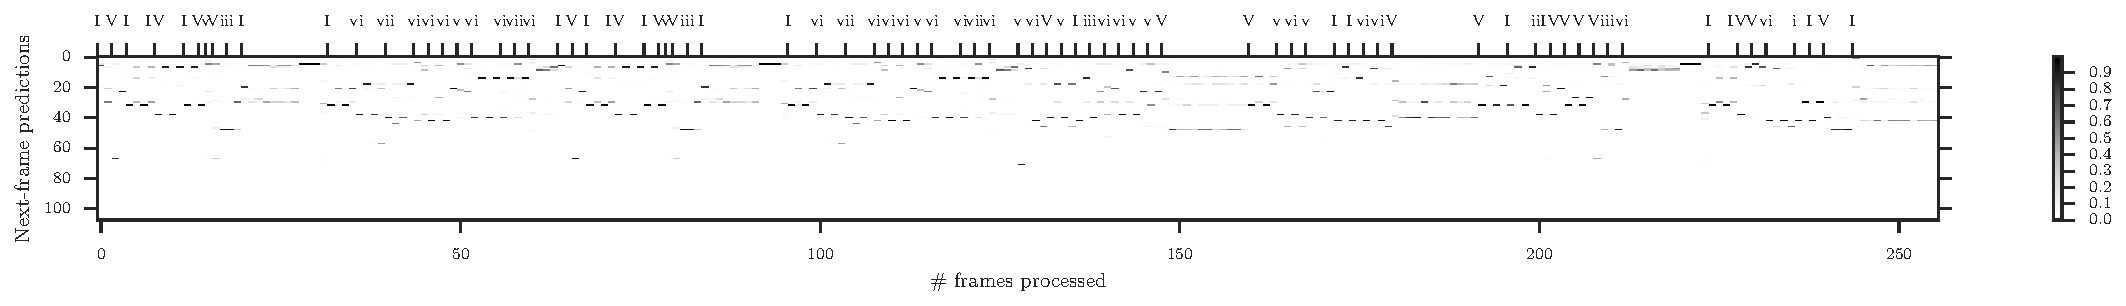
\includegraphics[width=1.0\linewidth]{model-analysis-chords-5.pdf}
    \caption{Neuron activations over time pooled over frames}
    \label{fig:model-analysis-frames}
\end{figure}

\subsection{Probabilistic piano roll: likely variations of the stimulus}

The bottom panel in \cref{fig:model-analysis-frames} shows the model's predictions
for tokens in the next frames, where the tokens are arranged according to (arbitrary)
index within the vocabulary. As the tokens correspond to pitches, they can be sorted
according to pitch to reconstruct a {\bf probabilistic piano roll}\citep{eck2008learning}
consisting of the model's sequence of next-frame predictions as it processes the input.

\mynote{Align these}
\begin{figure}[tb]
    \centering
    ~~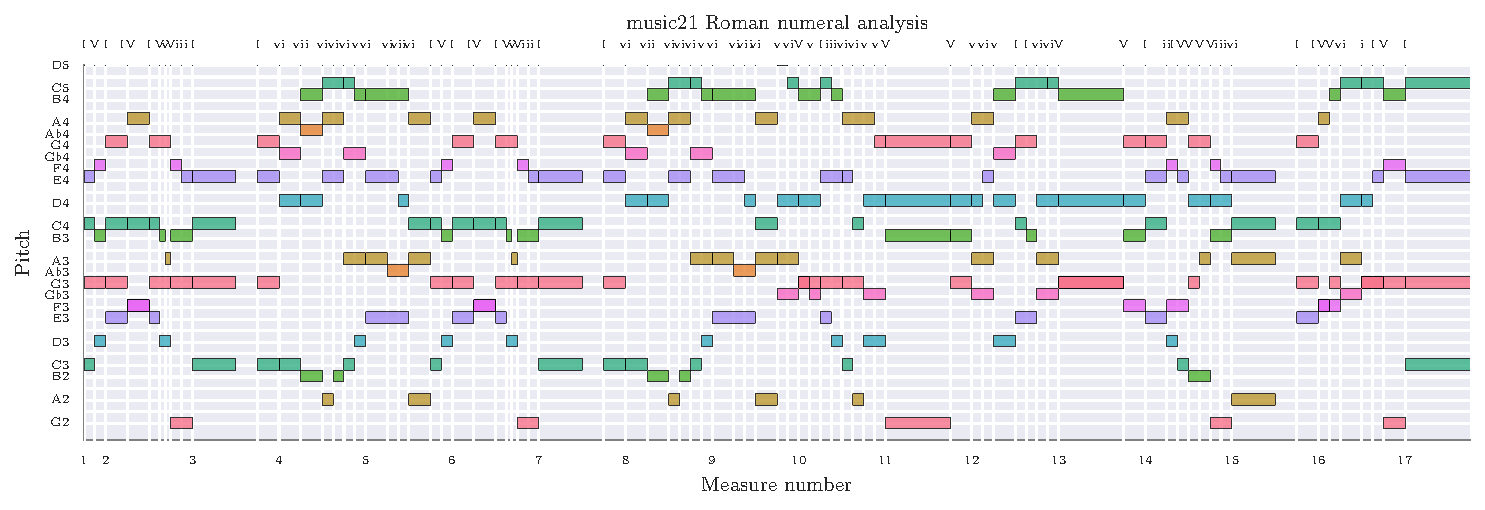
\includegraphics[width=0.99\linewidth]{model-analysis-input-piano-roll.pdf}
    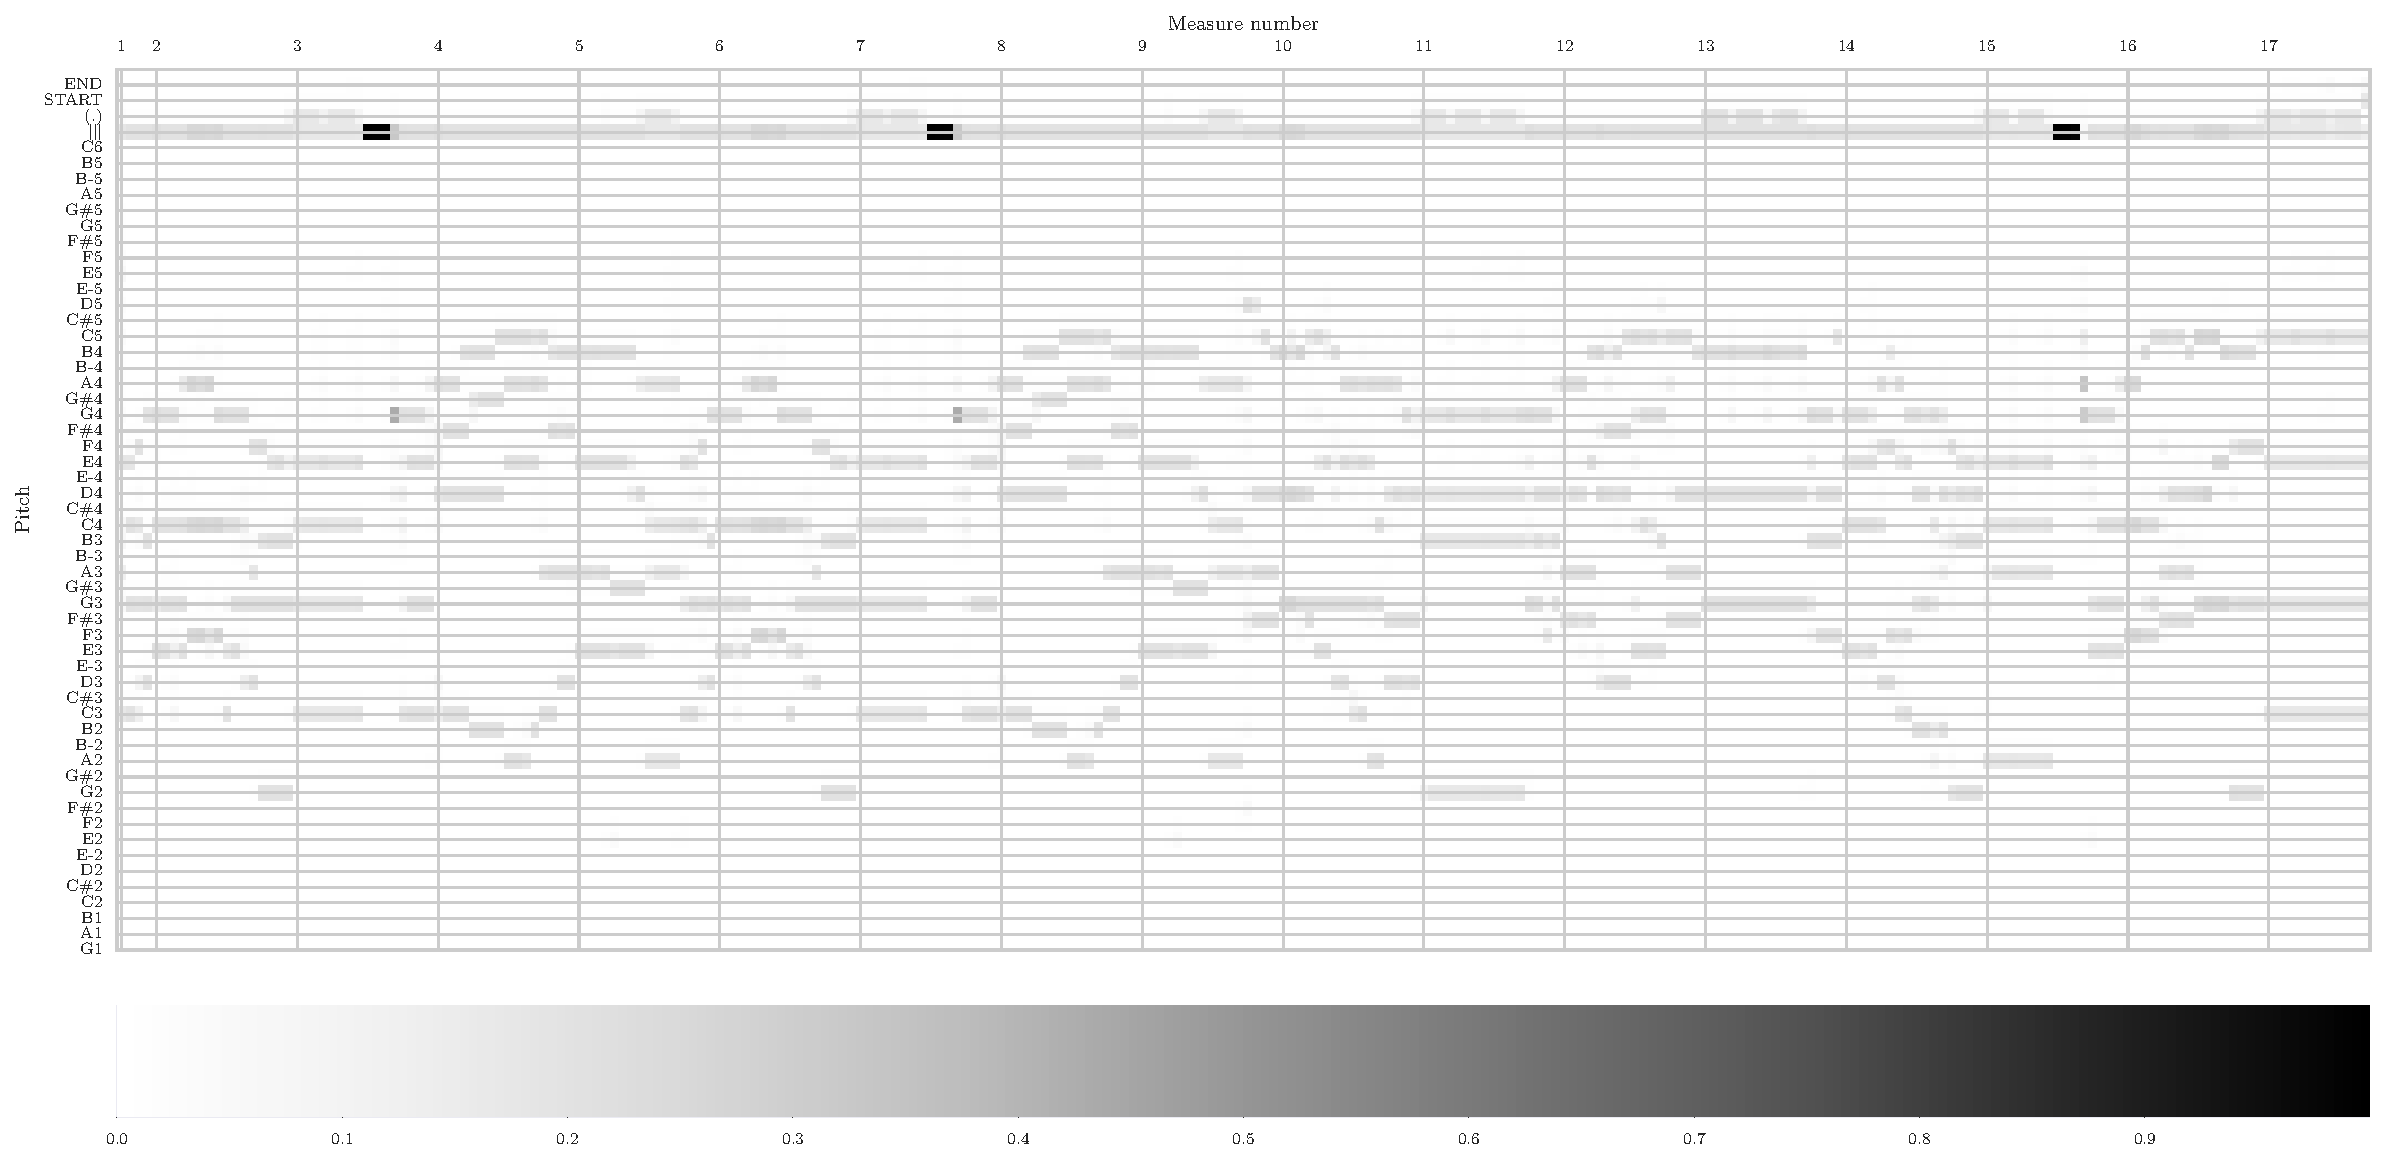
\includegraphics[trim={0 0 0 1.4cm},clip,width=1.0\linewidth]{model-analysis-probabilistic-piano-roll.pdf}
    \caption{Top: piano roll of stimulus (included for reference); Bottom: probabilistic piano roll}
    \label{fig:model-analysis-probabilistic-piano-roll}
\end{figure}

Notice that the probabilistic piano roll in
\cref{fig:model-analysis-probabilistic-piano-roll} closely resembles the
stimulus. This is unsurprising because the recurrent inputs are taken from the
stimulus rather than sampled from the model's predictions (a.k.a.
\citep{williams1989learning}), so a model which predicts to only continue holding
its input would produce a probabilistic piano roll identical to the stimulus
delayed by one frame.

Two interesting rows of \cref{fig:model-analysis-probabilistic-piano-roll}
are the rows corresponding to frame delimiters (fourth from top, ``|||'') and
fermatas (third from top ``(.)''). Notice that the predictions for chord
delimiters are particularly strong during rests. This is because rests are
encoded as empty frames, so the large probability values indicate that the
model has learned to prolong periods of rests. At the end of rest periods, the
model tends to assign probability across a wide range of notes, consistent with
the intuition that the possible notes occuring directly after a rest is less
constrained than \mynote{cite the intuition?} those occuring in the middle of a
phrase. Finally, notice that the probability assigned to fermatas is larger
near the ends of phrases, suggesting that the model has successfully learned
the concept of phrasing within music.

The probabilistic piano roll can be interpreted as variations on the stimulus
which the model finds likely and may serve as a useful computational tool for
generating likely chorale variations.

\subsection{Neurons specific to musical concepts}

Research in convolutional networks has shown that individual neurons within the
network oftentimes specialize and specifically detect certain high-level visual
features\mynote{Cite deconvolution}. Extending the analogy to musical data, we
might expect certain neurons within our learned model to act as specific
detectors to certain musical concepts.

To investigate this further, we look at the activations over time of individual
neurons within the LSTM memory cells. Our results confirm our hypothesis: we
discover certain neurons whose activities are correlated to specific motifs,
chord progression, and phrase structures. The activity profiles of these
neurons are shown in \cref{fig:model-analysis-cells-individual}.

\begin{figure}[tb]
    \centering
    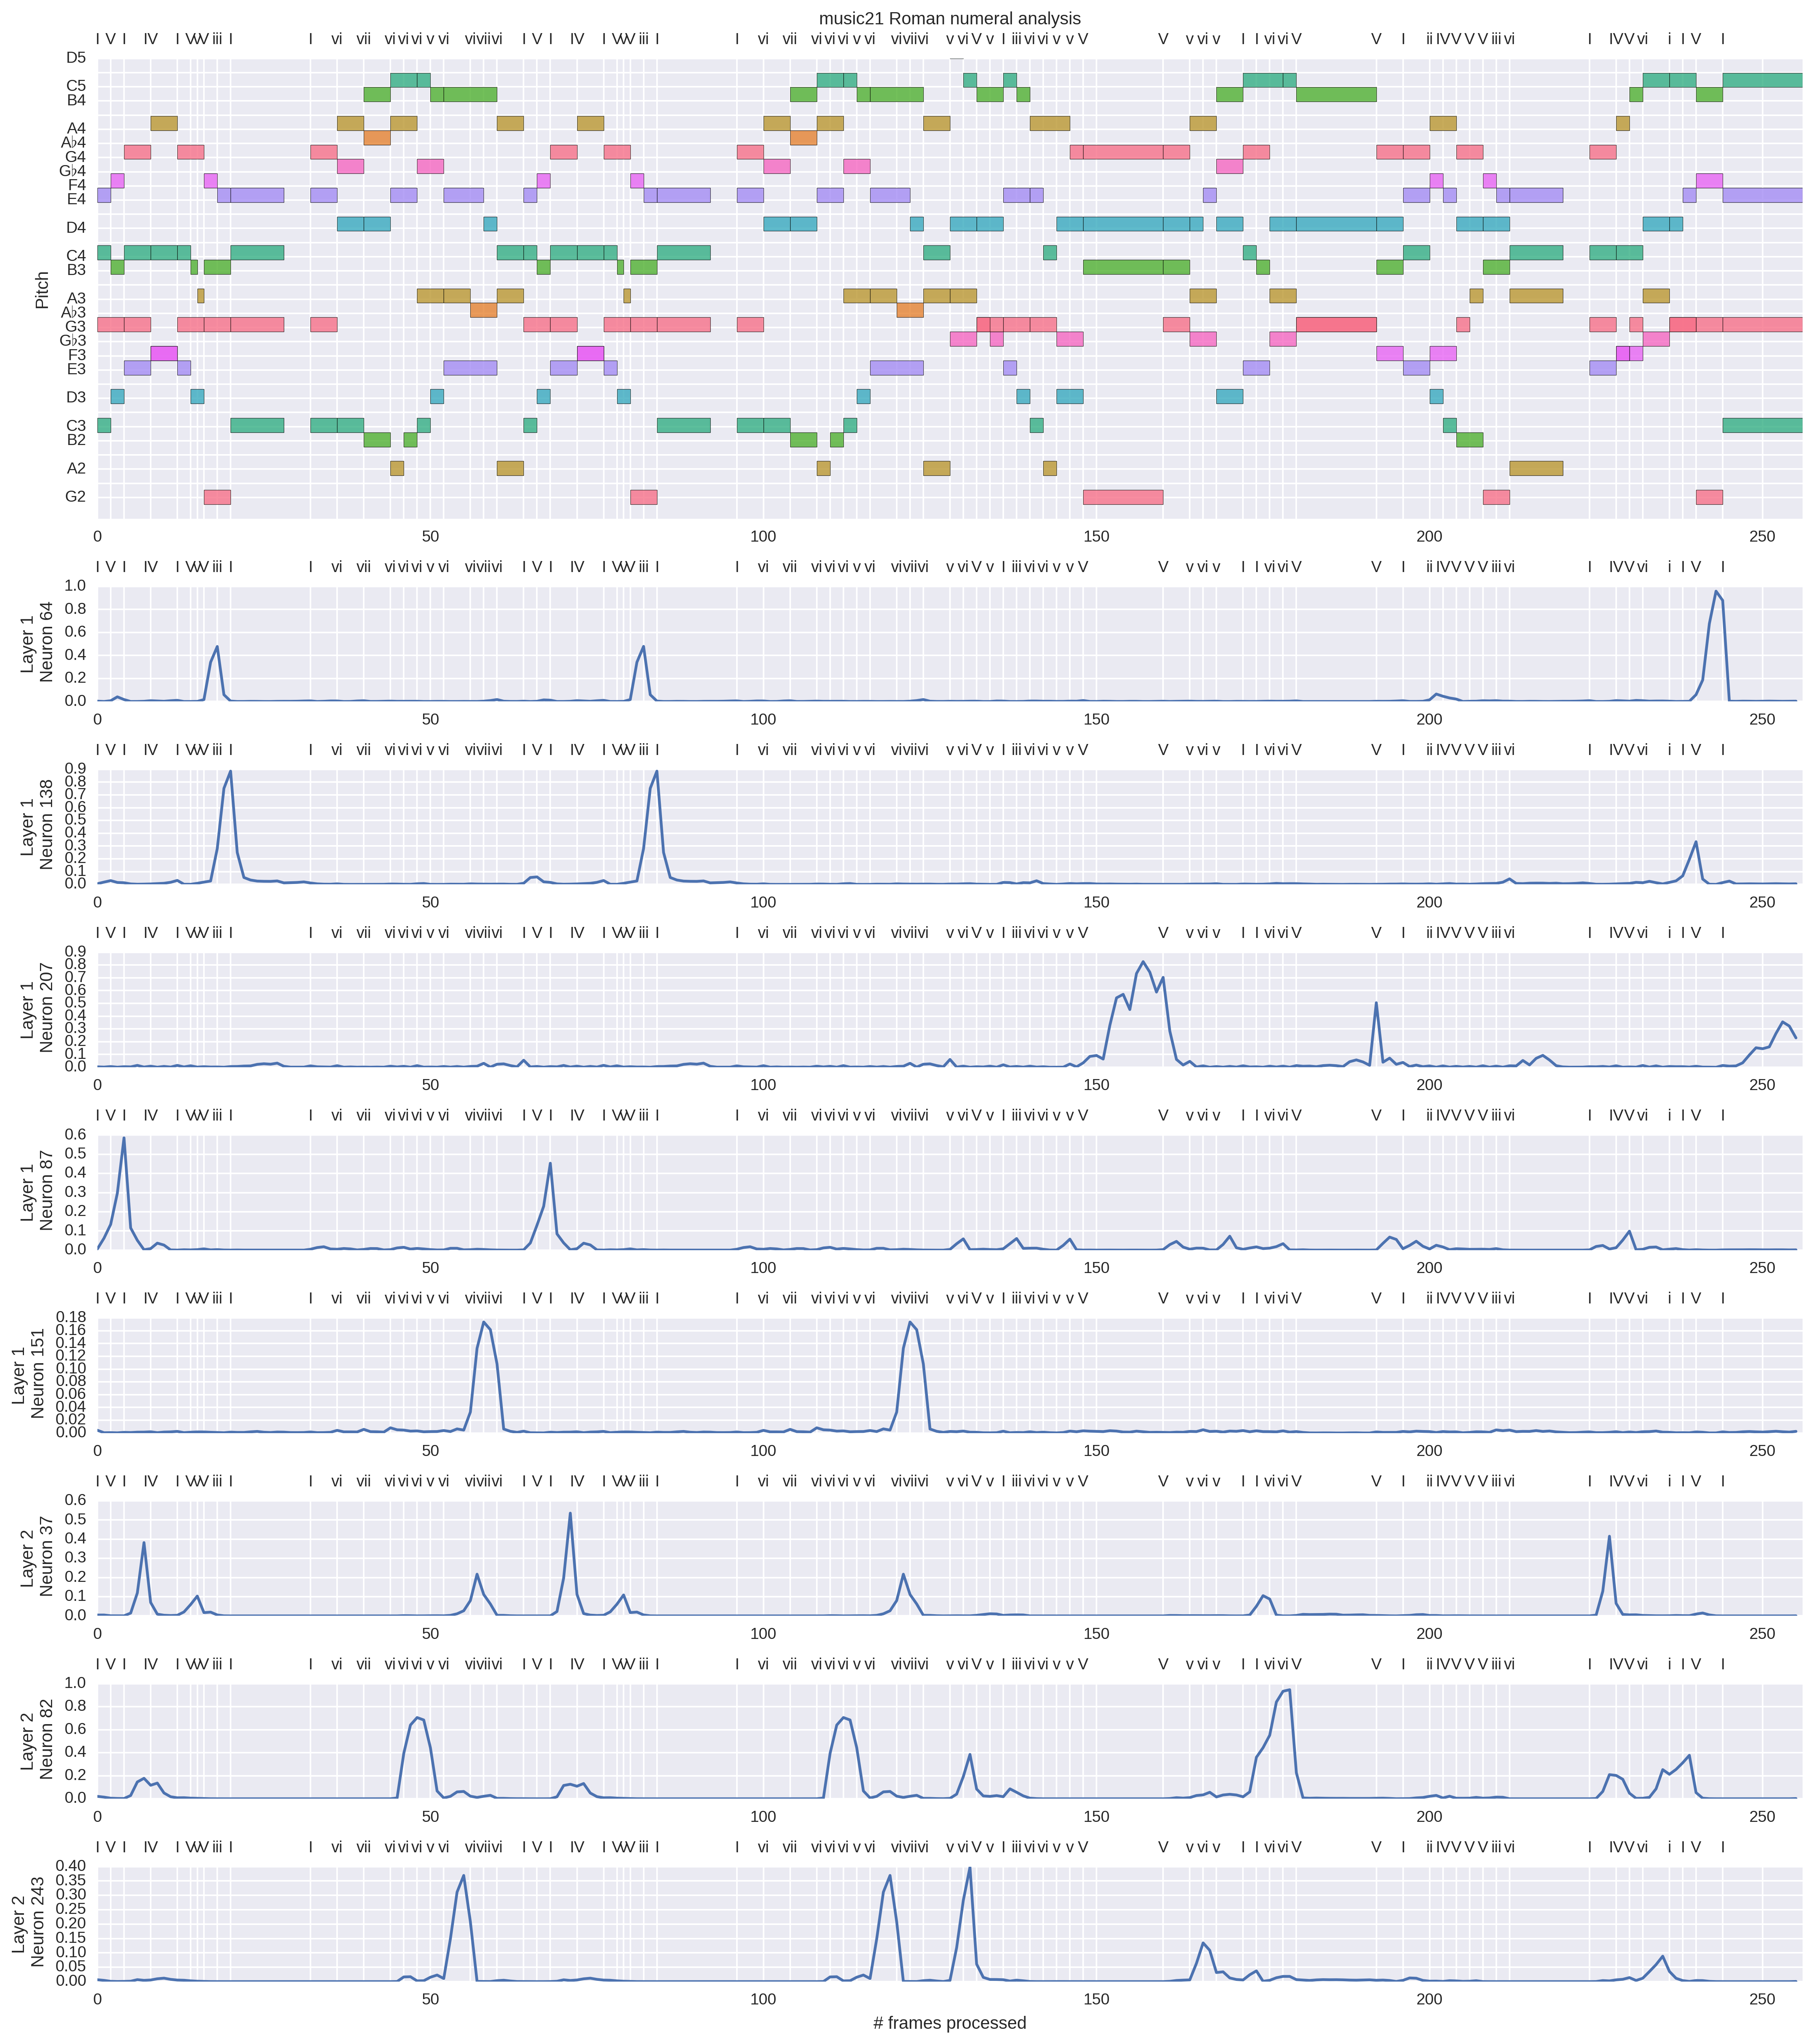
\includegraphics[width=1.0\linewidth]{model-analysis-cells-individual.png}
    \caption{Activation profiles of neurons within our model which have learned
    high-level musical concepts}
    \label{fig:model-analysis-cells-individual}
\end{figure}

For notational clarity, we will use the ordered tuple $(l,i)$ to refer to the
$i$th neuron in layer $l$.

The first three neurons ($(1,64)$, $(1,138)$, $(1,207)$) shown in the 2nd to
4th panel from top of \cref{fig:model-analysis-cells-individual} effectively
behave like cadence detectors. While they all exhibit activity when the
stimulus contains $V$ chords (\ie G-major). $(1,64)$ and $(1,138)$ are both
specific to perfect cadences (\ie $V -- I$ chord progressions) used to
conclude phrases and differ only in the chord inversions which they are most
sensitive to. In contrast, $(1,207)$ only exhibits activity for the $V$ chord
associated with the imperfect cadences near frames $150$ and $180$.

The next two neurons in \cref{fig:model-analysis-cells-individual}, $(1,87)$
and $(1,151)$, act as motif detectors. Activity in $(1,151)$ peaks when a $vi-vii-vi$
progression is present in the stimulus. $(1,87)$ exhibits large spikes on $I--V--I$,

$(2,37)$ exhibits less specificity, but has large spikes right before the $IV$ chord
in $I--IV$ chord progressions.

$(2,82)$ peaks at the top of an ascending harmonic progressions, right before a descending
major scale is to follow.

$(2, 243)$ is specific to $v -- vi$ progressions, with large spikes occuring at
the $v -- vi$ progressions near frames $55$, $120$, $130$, and a lower intensity spike at
$170$. Some activity is also observed for the $V -- vi$ around frame $230$ despite
the first chord being a major mode $V$ rather than minor $v$.

